%%%%%%%%%%%%%%%%%%%%%%%%%%%%%%%%%%%%%%%%%
% Paper Template 
% IOE Graduate Conference -- 2015
% Version 1.0
%
% Original author:
% Jayandra Raj Shrestha (jayandra@ioe.edu.np)
%
%%%%%%%%%%%%%%%%%%%%%%%%%%%%%%%%%%%%%%%%%

%----------------------------------------------------------------------------------------
%	PACKAGES AND OTHER DOCUMENT CONFIGURATIONS
%----------------------------------------------------------------------------------------

\documentclass[fleqn --11pt --twoside]{IOEGC2016} % Document font size and equations flushed left

\usepackage{float} %Required to force figures and tables to be placed as desired location
\usepackage{eucal}
\usepackage{devanagari} %Required for devnagari
\usepackage{multirow}

\PaperTitle{Improving Nepali Document Classification by Neural Network} % Article title

\Authors{Kaushal Kafle\textsuperscript{1} -- Diwas Sharma\textsuperscript{2} -- Aayush Subedi\textsuperscript{3} -- Arun Kr. Timalsina\textsuperscript{4}*} % Authors

\affiliation{\textsuperscript{1,2,3,4}\textit{Department of Electronics and Computer Engineering, IOE, Central Campus -- Pulchowk}} % Author 1,2,3, affiliation

\affiliation{*\textbf{Corresponding author}: t.arun@ioe.edu.np} % Corresponding author

%----------------------------------------------------------------------------------------
%	ABSTRACT
%----------------------------------------------------------------------------------------

\Abstract{Text classification is the task of classifying documents into predefined categories automatically. This paper compares different text classification methods based on their effectiveness on the Nepali language.
The lack of a standard Nepali corpus prompted for the creation of a manual data set by crawling various Nepali news sites. Nepali document classification is severely limited by the complexity of the language morphology. Document classification with word2vec employs neural network and simplifies the process of automatically categorizing Nepali documents while increasing the precision and recall over previously implemented techniques such as TF-IDF. Comparison of results between the models implemented with word2vec and that with TF-IDF shows that the word2vec model outperforms the TF-IDF model by 1.6 per cent in terms of F-score and 0.98 per cent in terms of accuracy. 
}

\Keywords{Support Vector Machine -- Text Classification -- Feature extraction -- TF-IDF -- Word2vec -- LSI -- Neural Network -- Nepali Corpus}


%----------------------------------------------------------------------------------------


\begin{document}
\setcounter{page}{1} %Will be changed by appropriate page number during final compilation
\flushbottom % Makes all text pages the same height
\maketitle % Print the title and abstract box
% \tableofcontents % Print the contents section
\thispagestyle{empty} % Removes page numbering from the first page

%----------------------------------------------------------------------------------------
%	ARTICLE CONTENTS
%----------------------------------------------------------------------------------------

%------------------------------------------------
% INTRODUCTION
%------------------------------------------------

\section*{Introduction}
\addcontentsline{toc}{section}{Introduction}
Automatic document classification has been a computationally challenging part of any language. It is even more challenging to algorithmically classify documents written in a language such as Nepali that is morphologically rich and structurally complex. This is also the primary reason why there is a lack of research done on Nepali language based text classifiers. A job of a text classifier is to automatically assign a given document to its pre-specified category. Documents may be classified based on a number of attributes such as document types (images, videos, texts, etc), their contents (stories, novels, poems, etc), their authors, etc. It has a wide range of applications such as spam filtering, document indexing, text filtering, news organization, etc. 
\par
The first problem of text classification is its feature extraction. It consists of acquiring a vector representation of the documents that can be used by the learning algorithm. Two methods, TF-IDF and word2vec \cite{mikolov2013distributed}, have been used for feature extraction in the paper. TF-IDF is a simple method that does not consider the order of the words in a sentence for classification purposes. Word2vec, however, is used when the contexts of the words are also to be taken into consideration. This paper focuses on the effects and efficiency of both the techniques along with their comparison with each other.
\par
Feature extraction using TF-IDF involves the calculation of IDF, which gives a measure of how important a word is to categorize a document. For example, the word `{\dn kro\symbol{'130}}' generally appears in documents related to business only, so its IDF measure is relatively high. On the other hand, word such as `{\dn ysr\symbol{70}}' has a high frequency in all documents so it is not particularly useful to determine which category a document should belong to. Hence, its IDF measure is low. 
\par
On the other hand, when the skip-gram architecture for word2vec is given any word, it calculates the probability of other words that occur in its surrounding within a specified window. For example, words such as `{\dn rAjDAn\symbol{70}}' and `{\dn up\symbol{40}ykA}' have a high probability of appearing nearby `{\dn kA\symbol{87}mA\symbol{88}O\symbol{32}}', but unrelated words like `{\dn DArA}' and `{\dn kml}' have a low probability. This is reflected on the representation of the words by word2vec. The word2vec algorithm in this classification model has been implemented using gensim.\cite{rehurek_lrec}
\par Classification of a document is done using either a supervised or an unsupervised learning method. SVM (Support Vector Machine) is an example of a supervised learning method. It is observed that SVMs consistently achieve good performance on text categorization tasks, outperforming existing methods substantially and significantly \cite{joachims1998text}. Using one-vs-all technique, SVM is used to build a model that can automatically assign input documents into any one of the categories based on the training data. The performance of the model largely depends on the configuration of the hyper-parameters of the training algorithm. Hyperopt \cite{bergstra2013making}, a Python library for serial and parallel optimization,  has been employed for calculating the optimal value of the regularization parameter (C) in SVM.
\section{Related Works}
Primarily, most of the works on text classification were based on English language. Apart from English language, some form of text classification system exists for European languages such as Italian, German, Spanish, etc. and Asian languages such as Arabic, Chinese and Japanese.
\par
Nepali is a morphologically rich language that has a fairly complicated orthography. Due to this, many language features has to be taken into consideration to build an efficient text classification model. Even so, commendable efforts have been made in the field of Nepali text classification using various methods.
\par
Shahi and Yadav analyse the effects of two classification techniques, the Naive Bayes and SVM, to develop a Mobile SMS spam filtering for Nepali text \cite{shahi2013mobile}.
Dangol and Timalsina implement various Nepali language specific features such as filtering stop-words, word replacements and removal of word suffices using Nepali language morphology to reduce the number of dimensions in Vector Space Model \cite{dangol2013features}. 
Similarly, Bam and Shahi classify rigid designators in Nepali text such as proper names, biological species and temporal expressions into some predefined categories which plays an important role in different fields such as Machine translation, Information Extraction, Question Answering System, etc. \cite{bam2014named}. 
\par
Currently, the number of commercial Nepali text classification system that categorizes the given documents into predefined specific categories based on their content is almost non-existent. This could be attributed to the fact that a reliable consistency and accuracy required at a commercial level hasn't been achieved because of the complexity of the Nepali language and also a lack of linguistic resources in Nepali such as a lack of generic stemmer, an accurate POS (Part-Of-Speech) tagger, stop-word filter, etc.
\par
The Nepali stemmer model developed by Bal and Shrestha \cite{bal2004morphological} is used for the purpose of this research.
\section{Methodology}
\subsection{Data Distribution}
A new Nepali corpus was built by collecting news documents from various popular Nepali news sites using a web crawler\footnote{\label{crawler}https://github.com/kad4/crawler} based on Scrapy\footnote{\label{scrapy}https://github.com/scrapy/scrapy}, a popular framework for extracting data from websites. 
A total of 13433 documents of different categories were collected from news portals such as Ratopati, Setopati, Onlinekhabar, Nepalipatra, etc. The collected dataset was further filtered and manual categorization was done to introduce more categories. 488 articles which didn't fall distinctly under any pre-specified category were sieved out. After the refining, 12945 articles were used during the research. The diverse nature of the collected data is shown in Table \ref{tab:data_distribution}. Finally, the filtered articles in their respective categories were used in the training and validation of the model.
\begin{table}[!ht]
\centering
    \caption{Data distribution}
    \begin{tabular}{|c|c|}
    \hline
        Category & No. of Documents \\ \hline
        automobiles & 283 \\ \hline
        finance & 837 \\ \hline
        crime & 491 \\ \hline
        employment & 206 \\ \hline
        entertainment & 2068 \\ \hline
        health & 1021 \\ \hline
        literature & 404 \\ \hline
        politics & 2879 \\ \hline
        society & 711 \\ \hline
        sports & 2052 \\ \hline
        technology & 1221 \\ \hline
        tourism & 772 \\ \hline
%        others & 488 \\ \hline
    \end{tabular}
    \label{tab:data_distribution}
\end{table}
\subsection{Stemmer}
A stemmer tailored for Nepali texts was used to tokenize the words in the dataset and strip them off of suffixes. These tokens were then subsequently passed to the feature extractors.
Example:

\begin{figure}[!h]
\centering
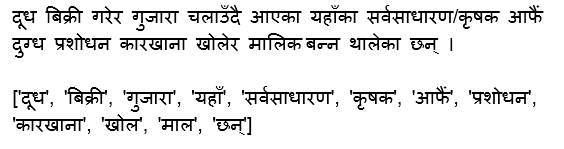
\includegraphics[width=\linewidth]{assets/example}
\end{figure}

\begin{figure}[!ht]
\centering
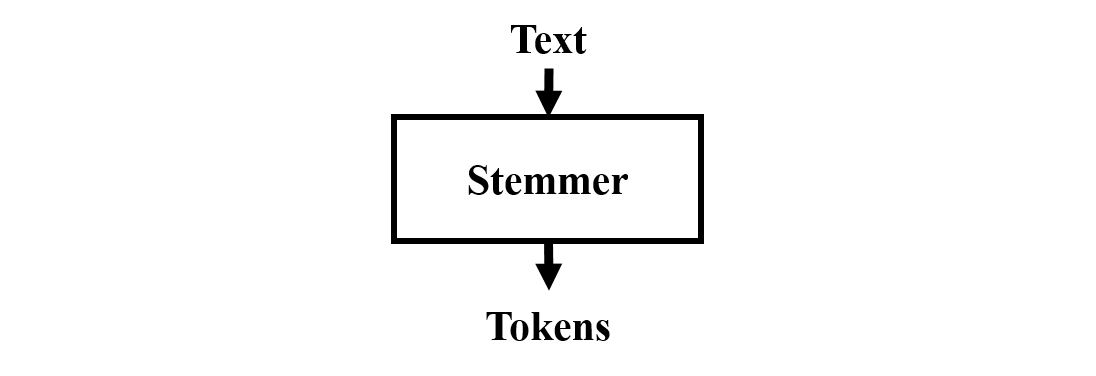
\includegraphics[width=\linewidth]{assets/stemmer}
\caption{Use of stemmer}
\label{fig:stemmer}
\end{figure}


%Input:
%कृषकले दूधबाट घिउ, छुर्पी, चिज, ललिलपलगायत सामग्री आफैं उत्पादन गरेर बिक्री गर्ने क्रम बढेको हो ।
%Output:
%['कृषक', 'दूध', 'घिउ', 'छुर्पी', 'चिज', 'सामग्री', 'आफैं', 'उत्पादन'

%'दूध बिक्री गरेर गुजारा चलाउँदै आएका यहाँका सर्वसाधारण/कृषक आफैं दुग्ध प्रशोधन कारखाना खोलेर मालिक बन्न थालेका छन् ।'

%Output:
%['दूध', 'बिक्री', 'गुजारा', 'यहाँ', 'सर्वसाधारण', 'कृषक', 'आफैं', 'प्रशोधन', 'कारखाना', 'खोल', 'माल', 'छन्']

\subsection{TF-IDF Feature Extractor}
The TF-IDF feature extractor works on the basis of the token frequencies it is fed. The algorithm with which it was implemented alongside the SVM classifier is as follows:
\begin{enumerate}
\item Preprocess dataset to obtain IDF for top 1000 stems
\item Tokenize and stem given text
\item Compute tf of stems obtained during preprocessing
\item Obtain a tf-idf vector representation of text by multiplying corresponding tf and idf
\end{enumerate}

\subsection{Word2Vec Feature Extractor}
The word2vec implementation used in this research uses a single hidden layer neural network having 300 neurons. The number of neurons in the input and the output layer is the number of tokens obtained after filtering out tokens having frequency less than 5 in the whole corpus. Following a typical skip-gram model, the word tokens are fed into the input neurons and for each word token, the corresponding set of words within a fixed window of size 10 that appear alongside the word tokens are fed to the output neurons. Tokens with a frequency of less than 5 are ignored. The negative sampling size is also kept at 5. Based on these two inputs, the hidden layer creates a matrix that keeps the information of the context of the words within the fixed window size. 
\begin{enumerate}
\item Train Neural Network for word2vec using skip-gram model with negative sampling
\item Tokenize and stem given text
\item Obtain the word vectors for individual words
\item Average the word vectors to obtain the vector representation for text
\end{enumerate}
 
\subsection{SVM Classifier}
The matrix acquired from the feature extractor is finally used by the SVM classifier.  It associates the matrix with the data label, or category which the text was from, and finally a trained classifier is achieved. This trained classifier is later used for predicting the category of unknown texts.\newline
Algorithm for training the classifier:
\begin{enumerate}
\item Obtain a list of labeled documents to be used for training
\item Perform feature extraction on each document to obtain a feature matrix
\item Compute the corresponding output matrix using document label
\item Use the feature matrix and output matrix to train the SVM
\item Perform hyperparameter optimization
\end{enumerate}
Algorithm for text categorization:
\begin{enumerate}
\item Perform feature extraction to obtain a feature vector
\item Feed corresponding vector into the trained SVM
\end{enumerate}
The flowchart of the overall system can be seen in figures \ref{fig:training} and \ref{fig:category}.
\begin{figure}[!ht]
\centering
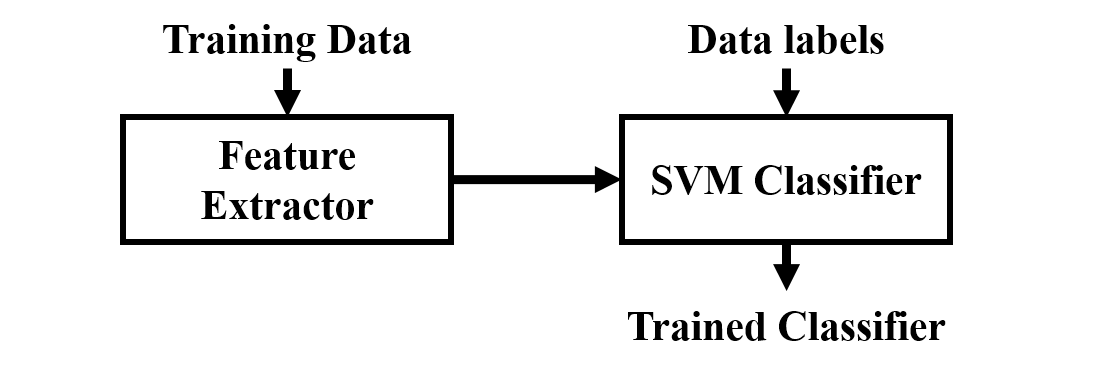
\includegraphics[width=\linewidth]{assets/training}
\caption{Training of classifier}
\label{fig:training}
\end{figure}
\begin{figure}[!ht]
\centering
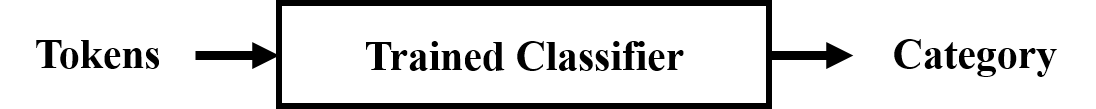
\includegraphics[width=\linewidth]{assets/category}
\caption{Category prediction using trained classifier}
\label{fig:category}
\end{figure}

% Maintain spacing add two lines above

\section{Evaluation}
\subsection{Optimization of Regularization Parameter (C)}
The performance of the classification algorithm, SVM, depends on its regularization parameter referred to as `C'. In order to automatically calculate the optimal value of `C' in each experiment cases, Hyperopt has been integrated into the training model. Equation \ref{eq:loss} is the cost function used by hyperopt to calculate C. Over the course of 10 experiment cases, hyperopt assigns a value for C and calculates the corresponding accuracy of each cases. The value of C that corresponds with the highest accuracy is used as the Regularization parameter C by SVM. 
\begin{equation}
loss= 1-accuracy
\label{eq:loss}
\end{equation} 
\begin{figure}[!ht]
\centering
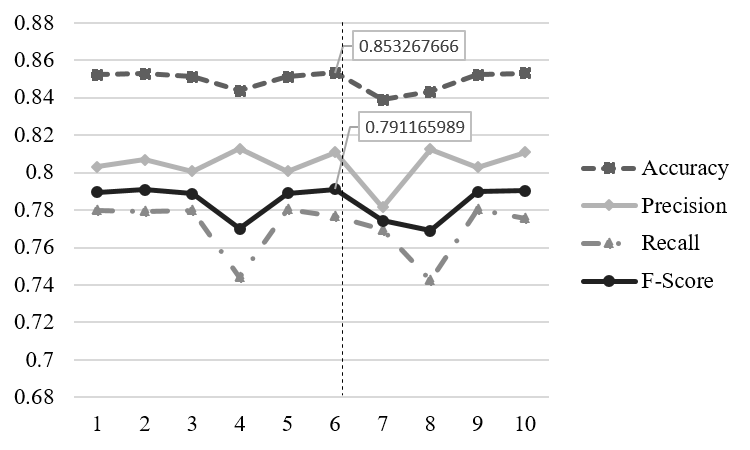
\includegraphics[width=\linewidth]{assets/hyperopt}
\caption{Hyper parameter optimization with hyperopt}
\label{fig:hyperopt}
\end{figure}
\subsection{Experiment procedure}
Each experiment consists of 10 sub-experiments which the hyperopt uses to obtain the optimal value for the regularization parameter, C. The experiments consisted of 5 fold cross validation in which test data size of 33.33 per cent of the total was used.
\subsection{Observation using TF-IDF}
The experiments have been first done on a model which uses TF-IDF method as its feature extractor. In its bare-bone form, TF-IDF uses all stems in the vocabulary for feature extraction. For optimum results, the model uses the 1000 most frequent stems for feature extraction. Because of this sheer number of stems fed into the SVM, it has a high dimensionality. Figure \ref{fig:performance_tf_idf} shows the variation of accuracy, precision, recall and F-Score over 5 experiments. The fluctuation can be attributed to the training data used and the optimum value of `C' calculated by hyperopt during each experiment.
\begin{figure}[!ht]
\centering
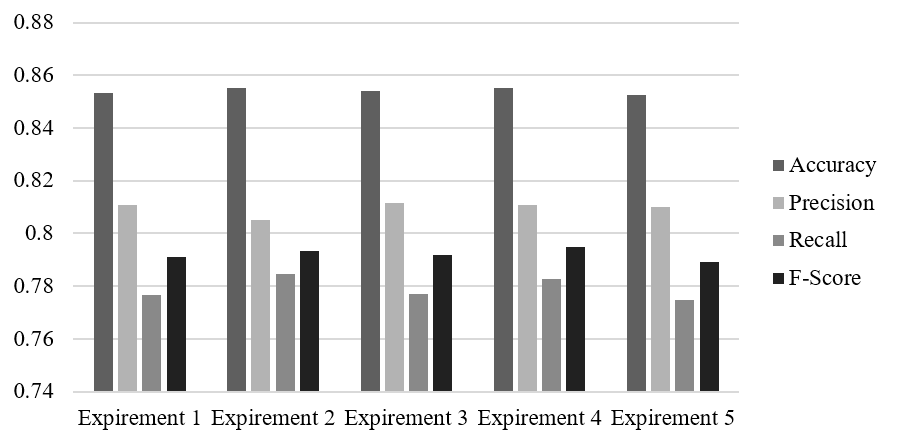
\includegraphics[width=\linewidth]{assets/performance_tf_idf}
\caption{Performance values obtained using TF-IDF}
\label{fig:performance_tf_idf}
\end{figure}
% \begin{table}[!ht]
% \centering
%     \caption{Mean performance values obtained using TF-IDF}
%     \begin{tabular}{|c|c|}
%         \hline
%         Performance Measures & Value \\ \hline
%         Accuracy & 0.854045276 \\ \hline
%         Precision & 0.809654627 \\ \hline
%         Recall & 0.779189265 \\ \hline
%         F-Score & 0.792013304 \\ \hline
%     \end{tabular}
%     \label{tab:performance_tf_idf}
% \end{table}
% \subsection{Observation using Latent Semantic Indexing}
% Dangol's model \cite{dangol2013features} uses cosine smilarity with TF-IDF for text classification and applies Latent Semantic Indexing (LSI) for dimensionality reduction. It uses other language specific features such as stopwords-filter, suffix-stripping, etc. to reduce the number of dimensions further.  Applying feature reduction techniques on the model helps to improve its efficiency in regards to the time and storage required to train it along with its performance measure.
% \begin{table}[!ht]
% \centering
%     \caption{Mean performance values obtained from experiments in reference}
%     \begin{tabular}{|c|c|}
%         \hline
%         Performance Measures & Value \\ \hline
%         Accuracy & 0.937694 \\ \hline
%         Precision & 0.795888 \\ \hline
%         Recall & 0.781929 \\ \hline
%         F-Score & 0.785624 \\ \hline
%     \end{tabular}
%     \label{tab:performance_dangol}
% \end{table}
% \par
% As a context-counting method, LSI is much more sensitive to the parameter choices \cite{baroni2014don}. Due to this, it has the tendency to produce much less desirable result when the parameter value is unsuitable. Even though impressive results were obtained using language-specific approaches such as stemmers, stop-word filters, etc. they rely heavily on in-depth knowledge of the dataset, language-specific semantics and performance tuning. 
% \par
% On the other hand, context-predicting method such as word2vec with the help of neural networks tend to be generally less sensitive to the parameter choices \cite{baroni2014don}. Given any dataset, they can churn out relatively better results when compared to the context-counting methods. The system model employed in this research uses word2vec as the feature extractor to specifically exploit this advantage of the neural networks in text classification. 
\subsection{Observation using word2vec}
%By being fundamentally different to LSI in its approach, 
Word2vec is a context-predicting method that uses neural networks for feature extraction and tends to be generally less sensitive to the parameter choices \cite{baroni2014don}. Given any dataset, it can churn out relatively better results when compared to the context-counting methods such as LSI. The system model employed in this research uses word2vec as the feature extractor to specifically exploit this advantage of the neural networks in text classification over commonly used TF-IDF model. Word2vec improves the dimensionality reduction in the training model which saves a large amount of stem overhead and processing time. Figure \ref{fig:performance_word2vec} shows the variation of accuracy, precision, recall and f-score over 5 experiments. The rise and fall of the values can be attributed to the dataset and the optimum value of `C' calculated by hyperopt during each experiment.
\begin{figure}[!ht]
\centering
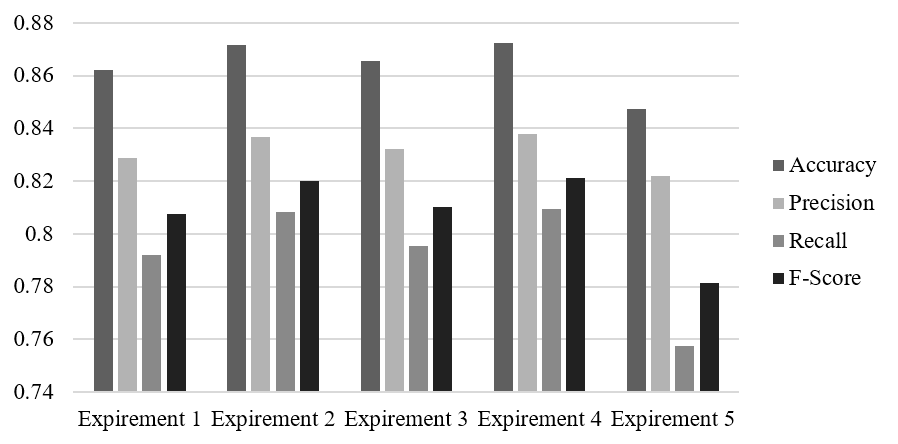
\includegraphics[width=\linewidth]{assets/performance_word2vec}
\caption{Performance values obtained using word2vec}
\label{fig:performance_word2vec}
\end{figure}
% 
% \begin{table}[!ht]
% \centering
%     \caption{Mean performance values obtained using word2vec}
%     \begin{tabular}{|c|c|}
%         \hline
%         Performance Measures & Value \\ \hline
%         Accuracy & 0.863845162 \\ \hline
%         Precision & 0.831501748 \\ \hline
%         Recall & 0.792444839 \\ \hline
%         F-Score & 0.808097445 \\ \hline
%     \end{tabular}
%     \label{tab:performance_word2vec}
% \end{table}
\subsection{Comparison of performance across models}
\begin{table}[!ht]
\centering
    \caption{Mean performance values comparison obtained from different methods}
    \begin{tabular}{|c|c|c|c|}
        \hline
        Measures & TF-IDF & word2vec \\ \hline
        Accuracy & 0.854045276 & 0.863845162 \\ \hline
        Precision & 0.809654627 & 0.831501748 \\ \hline
        Recall & 0.779189265 & 0.792444839 \\ \hline
        F-Score & 0.792013304 & 0.808097445 \\ \hline
    \end{tabular}
    \label{tab:performance}
\end{table}
\begin{figure}[!ht]
\centering
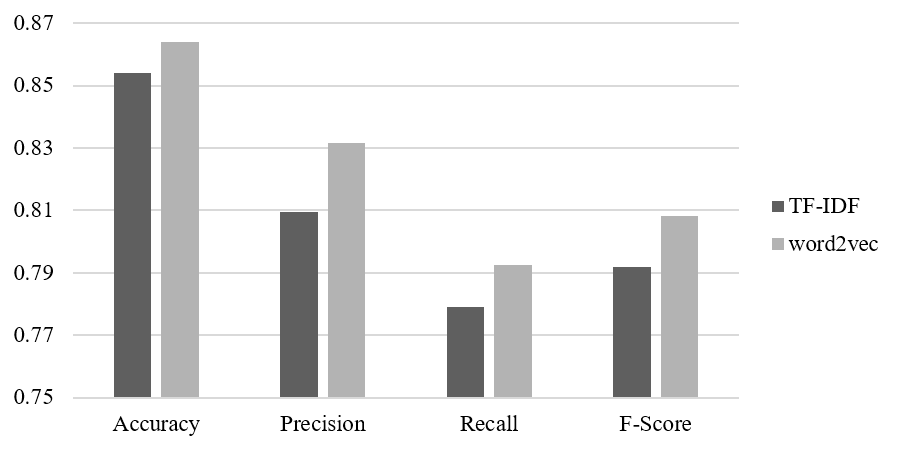
\includegraphics[width=\linewidth]{assets/comparison_nvo}
\caption{Performance comparison with reference}
\label{fig:comparison_nvo}
\end{figure}
Table \ref{tab:performance} shows the mean performance values that were obtained from both the models. Figure \ref{fig:comparison_nvo} is a graphical representation of the table that shows the variation of the performance measures. It indicates that the model with word2vec implementation has the highest Fscore value, and hence, the best overall performance.
\par The first model features a simplistic approach containing only the TF-IDF feature extractor along with SVM. while the second model employs the same classification algorithm, SVM, but uses a neural network-based feature extraction method word2vec. 
As figure \ref{fig:comparison_nvo} suggests, the mean accuracy of the models are 85.4 per cent and 86.4 per cent while their mean F-score are 79.2 per cent and 80.8 per cent respectively. Based on the comparison seen in figure \ref{fig:comparison_nvo}, the SVM model with word2vec improves on the precision and recall over the model with TF-IDF by 2.18 per cent and 1.33 per cent respectively. This results in the F-score of the word2vec model being superior to the TF-IDF method by 1.6 per cent.
%\par The measure of the classifier's accuracy doesn't always convey the efficiency of the model's performance satisfactorily. It is easily skewed by the unevenness of the data distribution among the categories. However, a better F-score which is the harmonic mean of precision and recall of the model is indicative of the fact that the model is more precise and has a complete prediction ability. Figure \ref{fig:comparison_nvo} shows that the SVM model with word2vec has a better precision and recall over the model with TF-IDF only by 2.18 per cent 1.33 per cent respectively. Similarly, the model has a better precision and recall of 3.56 per cent and 1.05 per cent respectively over the model with LSI. This results in the F-score of the word2vec model being superior to the TF-IDF only method by 1.6 per cent and the LSI method by 2.2 per cent. The proposed model with word2vec lags behind the LSI model only in terms of accuracy, but has a higher overall precision and recall, leading to a higher F-score. 


% \subsection{Performance of SVM on 20 newsgroup dataset}
% Rennie and Rifkin \cite{rennie2001improving} compare the performance of Naive Bayes and SVM on a multi class % text classification. In their experiments, they have trained a SVM on 20 newsgroup data-set and have achieved % an accuracy of 86.9 per cent by using one-vs-all technique.
\section{Conclusion}
The lack of research works and the complexity of Nepali as a language made it difficult to find reliable linguistic resources that made our task tedious. The nonexistence of a standard Nepali corpus led us to create our own corpus by crawling various Nepali news sites. However, after the completion of the classification model, there were encouraging results that neural network, particularly word2vec, brought to automatic Nepali document classification. 
\par
In this paper, parameters such as accuracy, precision, F-score and recall have been used to evaluate the efficiency of the models. The SVM model with TF-IDF as feature extraction had no integrated dimensionality reduction feauture. However, the model with SVM and word2vec outperforms it in terms of F-score by 1.6 per cent. The training model is also greatly simplified by employing a neural network for learning. It is also less sensitive external factors and parameters which helped to maintain a much consistent results of document categorization over all the experiments. 

%------------------------------------------------


%----------------------------------------------------------------------------------------
%	ACKNOWLEDGEMENT
%----------------------------------------------------------------------------------------
%\phantomsection
%\section*{Acknowledgments} % The \section*{} command stops section numbering

%\addcontentsline{toc}{section}{Acknowledgments} % Adds this section to the table of contents
%Authors would like to thank Dr. Arun Kr. Timalsina for his guidance and supervision throughout this research.


%----------------------------------------------------------------------------------------
%	REFERENCE LIST
%----------------------------------------------------------------------------------------
\phantomsection
\bibliographystyle{unsrt}
\bibliography{refs}

%----------------------------------------------------------------------------------------

\end{document}